\documentclass[11pt]{article}

\usepackage{graphicx}
\usepackage{framed}
\usepackage{hyperref}
\usepackage{listings}
\usepackage{xcolor}
\usepackage{caption}
\usepackage{subcaption}

\usepackage{booktabs}
\usepackage{amsmath}

\marginparwidth 0.5in 
\oddsidemargin 0.25in 
\evensidemargin 0.25in 
\marginparsep 0.25in
\topmargin 0.25in 
\textwidth=6in
\textheight=8in

\definecolor{codegreen}{rgb}{0,0.6,0}
\definecolor{codegray}{rgb}{0.5,0.5,0.5}
\definecolor{codepurple}{rgb}{0.58,0,0.82}
\definecolor{backcolor}{rgb}{0.95,0.95,0.95}

\lstset{
  backgroundcolor=\color{backcolor}, % Set background color
  commentstyle=\color{codegreen}, % Style for comments
  keywordstyle=\color{magenta}, % Style for keywords
  numberstyle=\tiny\color{codegray}, % Style for line numbers
  stringstyle=\color{codepurple}, % Style for strings
  basicstyle=\ttfamily\footnotesize, % Basic font style and size
  breakatwhitespace=false, % Don't break lines at whitespace only
  breaklines=true, % Enable line breaking
  captionpos=b, % Caption position (bottom)
  keepspaces=true, % Keep spaces
  numbers=left, % Show line numbers on the left
  numbersep=5pt, % Separation of numbers from code
  showspaces=false, % Don't show spaces as visible characters
  showstringspaces=false, % Don't show spaces in strings
  showtabs=false, % Don't show tabs as visible characters
  tabsize=2, % Tab size
  language=Python % Specify the language
}


\begin{document}
\hfill\vbox{\hbox{Jude Shin, Torrey Zachs}
		\hbox{CSC 321, Section 07}	
		\hbox{Module 6}	
		\hbox{\today}}\par

\bigskip
\centerline{\Large\bf Lab 07: Leviathan and Microcorruption}\par
\bigskip

This lab completes two CTFs: Leviathan and Microcorruption.

All the code can be found in our remote \href{https://github.com/jude-shin/CSC\_321}{GitHub} repository.

% ============================================================================

\section*{6a: Leviathan}
\subsection*{Part 1}
\subsection*{Part 2}
\subsection*{Part 3}
\subsection*{Part 4}
\subsection*{Part 5}

\verb|cat helloworld.txt|



\section*{6b: Microcorruption}
\subsection*{Part 1}
\subsection*{Part 2}
\subsection*{Part 3}
\subsection*{Part 4}
\subsection*{Part 5}

\subsection*{Screenshot of our Progress}
\begin{figure}[!ht]
	\centering
	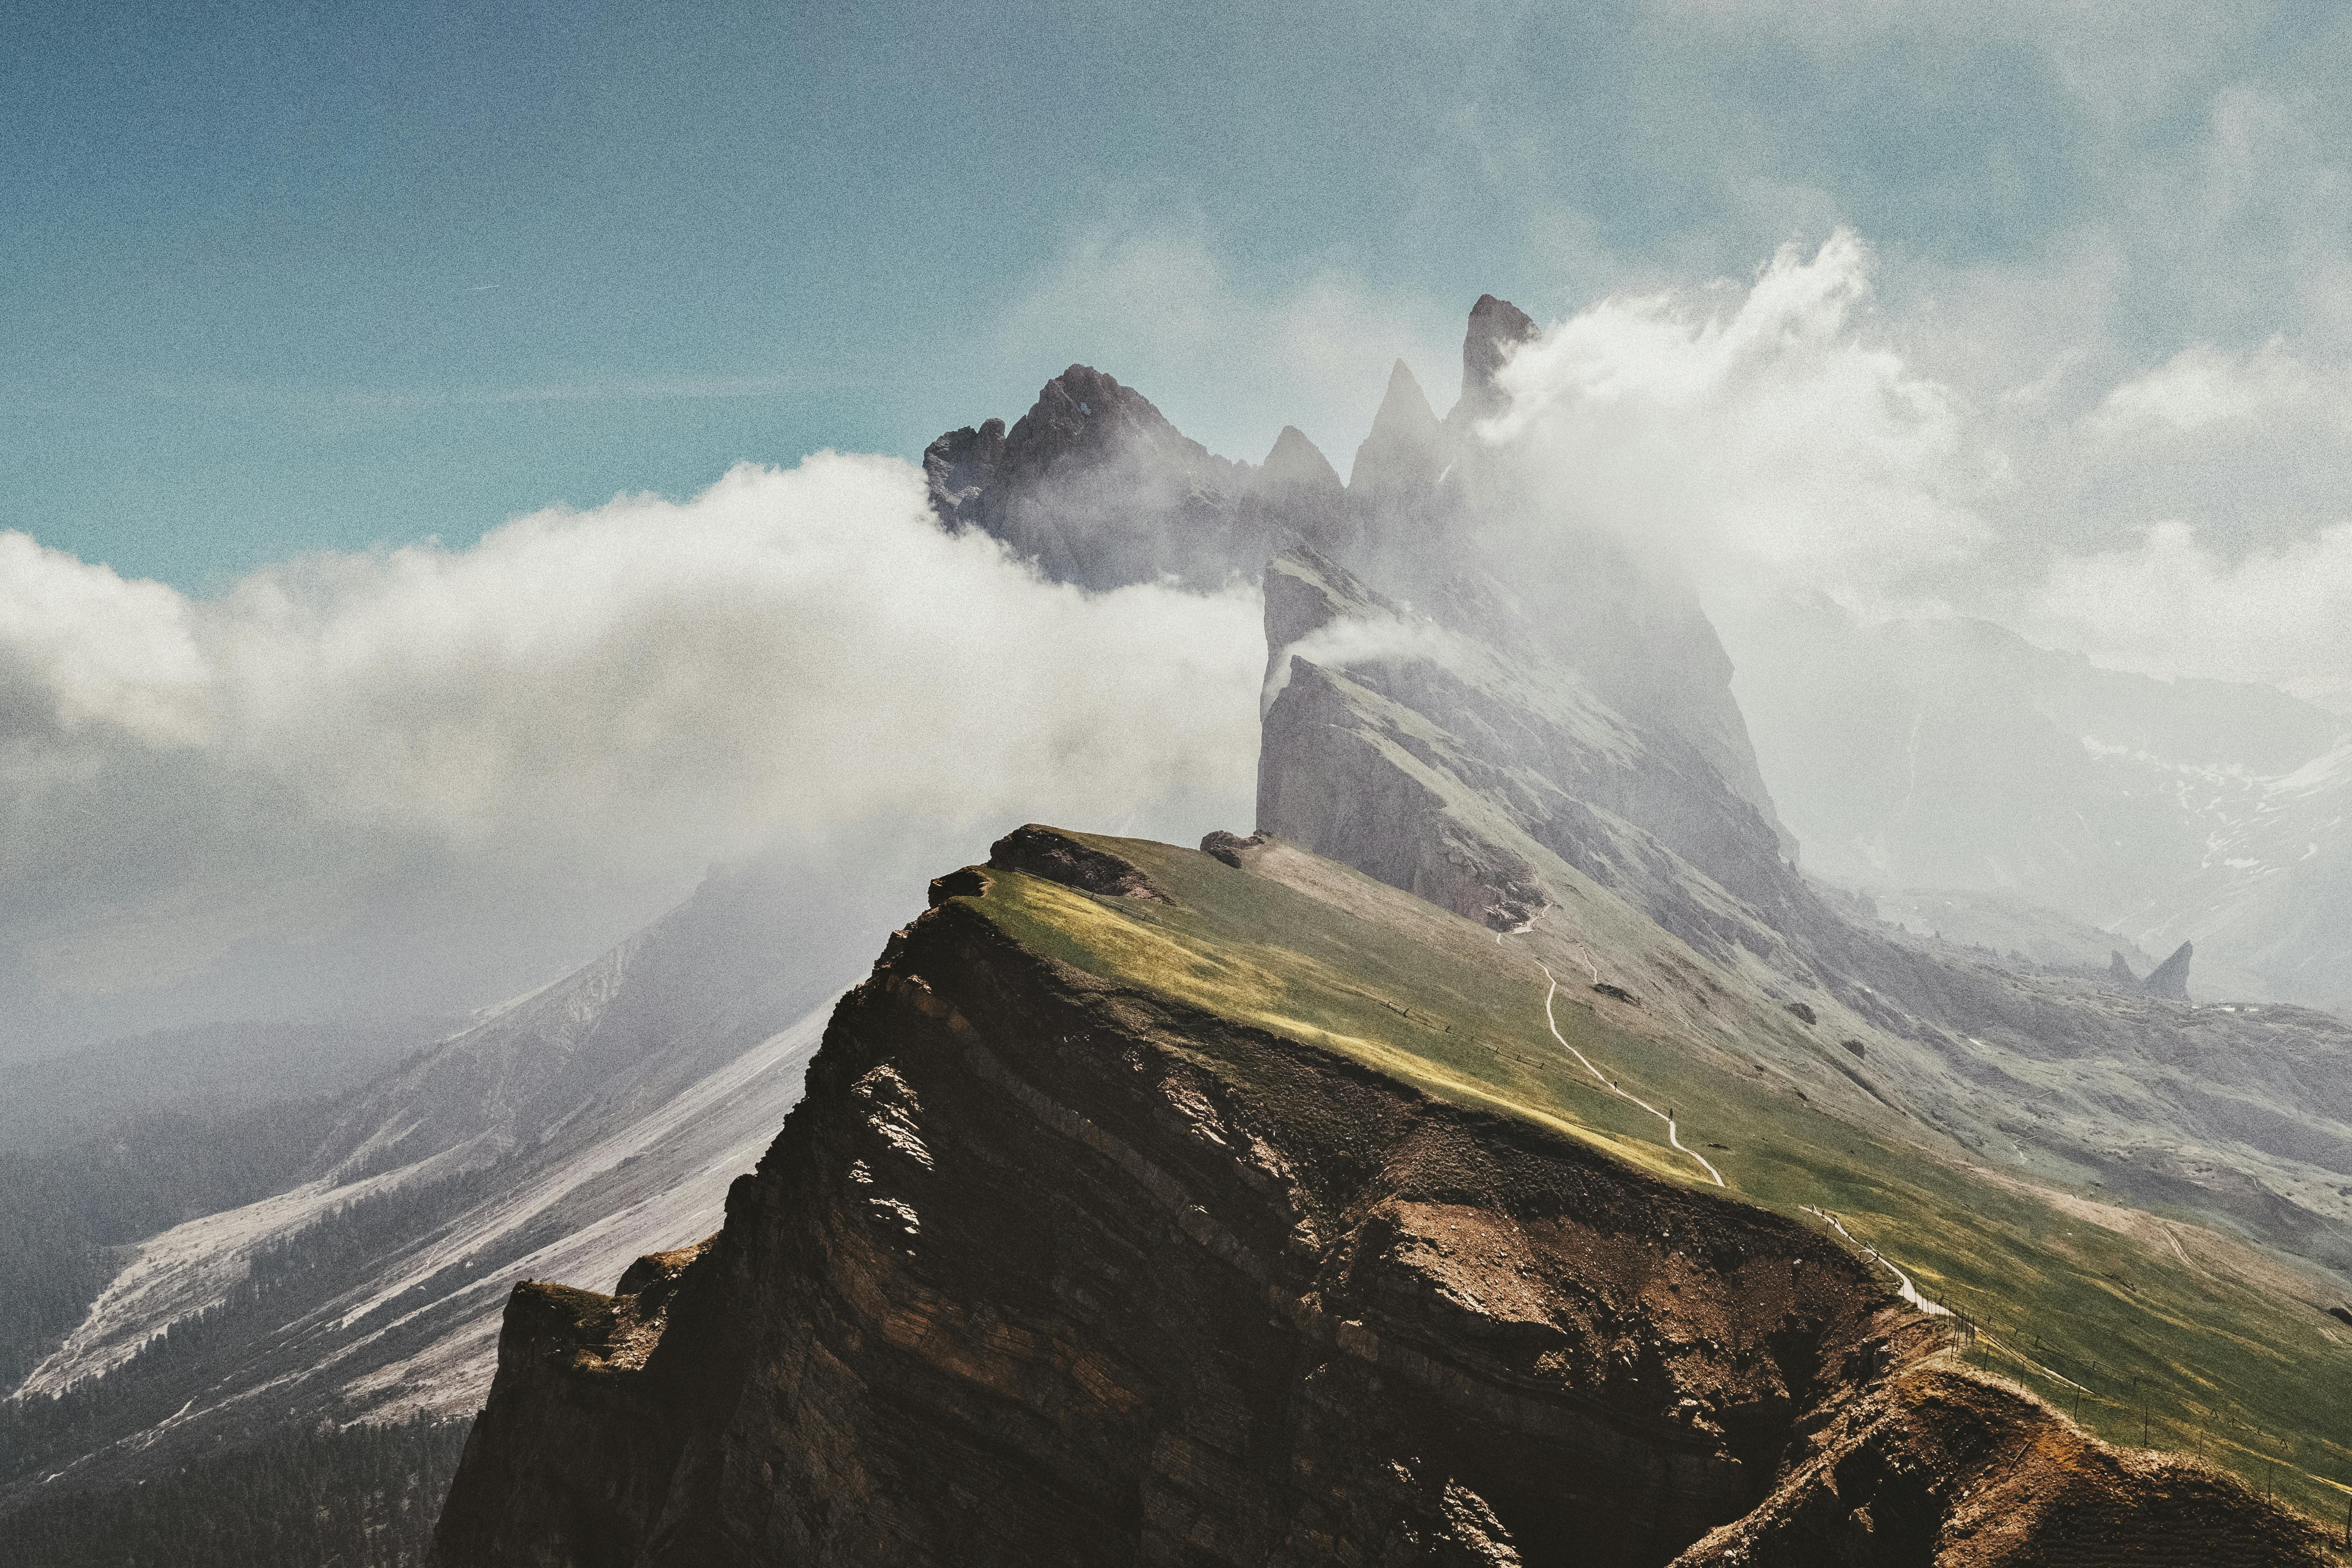
\includegraphics[width=1.0\textwidth]{./assets/progress.jpg}
	\caption{Screenshot of the Progress}
	\label{fig:progress}
\end{figure}

\end{document}
